\documentclass[twoside]{article}

\usepackage{aistats2021}
% If your paper is accepted, change the options for the package
% aistats2021 as follows:
%
%\usepackage[accepted]{aistats2021}
%
% This option will print headings for the title of your paper and
% headings for the authors names, plus a copyright note at the end of
% the first column of the first page.

% If you set papersize explicitly, activate the following three lines:
%\special{papersize = 8.5in, 11in}
%\setlength{\pdfpageheight}{11in}
%\setlength{\pdfpagewidth}{8.5in}

% If you use natbib package, activate the following three lines:
%\usepackage[round]{natbib}
%\renewcommand{\bibname}{References}
%\renewcommand{\bibsection}{\subsubsection*{\bibname}}

% If you use BibTeX in apalike style, activate the following line:

%%%%% NEW MATH DEFINITIONS %%%%%

\usepackage{amsmath,amsfonts,bm}

% Mark sections of captions for referring to divisions of figures
\newcommand{\figleft}{{\em (Left)}}
\newcommand{\figcenter}{{\em (Center)}}
\newcommand{\figright}{{\em (Right)}}
\newcommand{\figtop}{{\em (Top)}}
\newcommand{\figbottom}{{\em (Bottom)}}
\newcommand{\captiona}{{\em (a)}}
\newcommand{\captionb}{{\em (b)}}
\newcommand{\captionc}{{\em (c)}}
\newcommand{\captiond}{{\em (d)}}

% Highlight a newly defined term
\newcommand{\newterm}[1]{{\bf #1}}


% Figure reference, lower-case.
\def\figref#1{figure~\ref{#1}}
% Figure reference, capital. For start of sentence
\def\Figref#1{Figure~\ref{#1}}
\def\twofigref#1#2{figures \ref{#1} and \ref{#2}}
\def\quadfigref#1#2#3#4{figures \ref{#1}, \ref{#2}, \ref{#3} and \ref{#4}}
% Section reference, lower-case.
\def\secref#1{section~\ref{#1}}
% Section reference, capital.
\def\Secref#1{Section~\ref{#1}}
% Reference to two sections.
\def\twosecrefs#1#2{sections \ref{#1} and \ref{#2}}
% Reference to three sections.
\def\secrefs#1#2#3{sections \ref{#1}, \ref{#2} and \ref{#3}}
% Reference to an equation, lower-case.
\def\eqref#1{equation~\ref{#1}}
% Reference to an equation, upper case
\def\Eqref#1{Equation~\ref{#1}}
% A raw reference to an equation---avoid using if possible
\def\plaineqref#1{\ref{#1}}
% Reference to a chapter, lower-case.
\def\chapref#1{chapter~\ref{#1}}
% Reference to an equation, upper case.
\def\Chapref#1{Chapter~\ref{#1}}
% Reference to a range of chapters
\def\rangechapref#1#2{chapters\ref{#1}--\ref{#2}}
% Reference to an algorithm, lower-case.
\def\algref#1{algorithm~\ref{#1}}
% Reference to an algorithm, upper case.
\def\Algref#1{Algorithm~\ref{#1}}
\def\twoalgref#1#2{algorithms \ref{#1} and \ref{#2}}
\def\Twoalgref#1#2{Algorithms \ref{#1} and \ref{#2}}
% Reference to a part, lower case
\def\partref#1{part~\ref{#1}}
% Reference to a part, upper case
\def\Partref#1{Part~\ref{#1}}
\def\twopartref#1#2{parts \ref{#1} and \ref{#2}}

\def\ceil#1{\lceil #1 \rceil}
\def\floor#1{\lfloor #1 \rfloor}
\def\1{\bm{1}}
\newcommand{\train}{\mathcal{D}}
\newcommand{\valid}{\mathcal{D_{\mathrm{valid}}}}
\newcommand{\test}{\mathcal{D_{\mathrm{test}}}}

\def\eps{{\epsilon}}


% Random variables
\def\reta{{\textnormal{$\eta$}}}
\def\ra{{\textnormal{a}}}
\def\rb{{\textnormal{b}}}
\def\rc{{\textnormal{c}}}
\def\rd{{\textnormal{d}}}
\def\re{{\textnormal{e}}}
\def\rf{{\textnormal{f}}}
\def\rg{{\textnormal{g}}}
\def\rh{{\textnormal{h}}}
\def\ri{{\textnormal{i}}}
\def\rj{{\textnormal{j}}}
\def\rk{{\textnormal{k}}}
\def\rl{{\textnormal{l}}}
% rm is already a command, just don't name any random variables m
\def\rn{{\textnormal{n}}}
\def\ro{{\textnormal{o}}}
\def\rp{{\textnormal{p}}}
\def\rq{{\textnormal{q}}}
\def\rr{{\textnormal{r}}}
\def\rs{{\textnormal{s}}}
\def\rt{{\textnormal{t}}}
\def\ru{{\textnormal{u}}}
\def\rv{{\textnormal{v}}}
\def\rw{{\textnormal{w}}}
\def\rx{{\textnormal{x}}}
\def\ry{{\textnormal{y}}}
\def\rz{{\textnormal{z}}}

% Random vectors
\def\rvepsilon{{\mathbf{\epsilon}}}
\def\rvtheta{{\mathbf{\theta}}}
\def\rva{{\mathbf{a}}}
\def\rvb{{\mathbf{b}}}
\def\rvc{{\mathbf{c}}}
\def\rvd{{\mathbf{d}}}
\def\rve{{\mathbf{e}}}
\def\rvf{{\mathbf{f}}}
\def\rvg{{\mathbf{g}}}
\def\rvh{{\mathbf{h}}}
\def\rvu{{\mathbf{i}}}
\def\rvj{{\mathbf{j}}}
\def\rvk{{\mathbf{k}}}
\def\rvl{{\mathbf{l}}}
\def\rvm{{\mathbf{m}}}
\def\rvn{{\mathbf{n}}}
\def\rvo{{\mathbf{o}}}
\def\rvp{{\mathbf{p}}}
\def\rvq{{\mathbf{q}}}
\def\rvr{{\mathbf{r}}}
\def\rvs{{\mathbf{s}}}
\def\rvt{{\mathbf{t}}}
\def\rvu{{\mathbf{u}}}
\def\rvv{{\mathbf{v}}}
\def\rvw{{\mathbf{w}}}
\def\rvx{{\mathbf{x}}}
\def\rvy{{\mathbf{y}}}
\def\rvz{{\mathbf{z}}}

% Elements of random vectors
\def\erva{{\textnormal{a}}}
\def\ervb{{\textnormal{b}}}
\def\ervc{{\textnormal{c}}}
\def\ervd{{\textnormal{d}}}
\def\erve{{\textnormal{e}}}
\def\ervf{{\textnormal{f}}}
\def\ervg{{\textnormal{g}}}
\def\ervh{{\textnormal{h}}}
\def\ervi{{\textnormal{i}}}
\def\ervj{{\textnormal{j}}}
\def\ervk{{\textnormal{k}}}
\def\ervl{{\textnormal{l}}}
\def\ervm{{\textnormal{m}}}
\def\ervn{{\textnormal{n}}}
\def\ervo{{\textnormal{o}}}
\def\ervp{{\textnormal{p}}}
\def\ervq{{\textnormal{q}}}
\def\ervr{{\textnormal{r}}}
\def\ervs{{\textnormal{s}}}
\def\ervt{{\textnormal{t}}}
\def\ervu{{\textnormal{u}}}
\def\ervv{{\textnormal{v}}}
\def\ervw{{\textnormal{w}}}
\def\ervx{{\textnormal{x}}}
\def\ervy{{\textnormal{y}}}
\def\ervz{{\textnormal{z}}}

% Random matrices
\def\rmA{{\mathbf{A}}}
\def\rmB{{\mathbf{B}}}
\def\rmC{{\mathbf{C}}}
\def\rmD{{\mathbf{D}}}
\def\rmE{{\mathbf{E}}}
\def\rmF{{\mathbf{F}}}
\def\rmG{{\mathbf{G}}}
\def\rmH{{\mathbf{H}}}
\def\rmI{{\mathbf{I}}}
\def\rmJ{{\mathbf{J}}}
\def\rmK{{\mathbf{K}}}
\def\rmL{{\mathbf{L}}}
\def\rmM{{\mathbf{M}}}
\def\rmN{{\mathbf{N}}}
\def\rmO{{\mathbf{O}}}
\def\rmP{{\mathbf{P}}}
\def\rmQ{{\mathbf{Q}}}
\def\rmR{{\mathbf{R}}}
\def\rmS{{\mathbf{S}}}
\def\rmT{{\mathbf{T}}}
\def\rmU{{\mathbf{U}}}
\def\rmV{{\mathbf{V}}}
\def\rmW{{\mathbf{W}}}
\def\rmX{{\mathbf{X}}}
\def\rmY{{\mathbf{Y}}}
\def\rmZ{{\mathbf{Z}}}

% Elements of random matrices
\def\ermA{{\textnormal{A}}}
\def\ermB{{\textnormal{B}}}
\def\ermC{{\textnormal{C}}}
\def\ermD{{\textnormal{D}}}
\def\ermE{{\textnormal{E}}}
\def\ermF{{\textnormal{F}}}
\def\ermG{{\textnormal{G}}}
\def\ermH{{\textnormal{H}}}
\def\ermI{{\textnormal{I}}}
\def\ermJ{{\textnormal{J}}}
\def\ermK{{\textnormal{K}}}
\def\ermL{{\textnormal{L}}}
\def\ermM{{\textnormal{M}}}
\def\ermN{{\textnormal{N}}}
\def\ermO{{\textnormal{O}}}
\def\ermP{{\textnormal{P}}}
\def\ermQ{{\textnormal{Q}}}
\def\ermR{{\textnormal{R}}}
\def\ermS{{\textnormal{S}}}
\def\ermT{{\textnormal{T}}}
\def\ermU{{\textnormal{U}}}
\def\ermV{{\textnormal{V}}}
\def\ermW{{\textnormal{W}}}
\def\ermX{{\textnormal{X}}}
\def\ermY{{\textnormal{Y}}}
\def\ermZ{{\textnormal{Z}}}

% Vectors
\def\vzero{{\bm{0}}}
\def\vone{{\bm{1}}}
\def\vmu{{\bm{\mu}}}
\def\vtheta{{\bm{\theta}}}
\def\va{{\bm{a}}}
\def\vb{{\bm{b}}}
\def\vc{{\bm{c}}}
\def\vd{{\bm{d}}}
\def\ve{{\bm{e}}}
\def\vf{{\bm{f}}}
\def\vg{{\bm{g}}}
\def\vh{{\bm{h}}}
\def\vi{{\bm{i}}}
\def\vj{{\bm{j}}}
\def\vk{{\bm{k}}}
\def\vl{{\bm{l}}}
\def\vm{{\bm{m}}}
\def\vn{{\bm{n}}}
\def\vo{{\bm{o}}}
\def\vp{{\bm{p}}}
\def\vq{{\bm{q}}}
\def\vr{{\bm{r}}}
\def\vs{{\bm{s}}}
\def\vt{{\bm{t}}}
\def\vu{{\bm{u}}}
\def\vv{{\bm{v}}}
\def\vw{{\bm{w}}}
\def\vx{{\bm{x}}}
\def\vy{{\bm{y}}}
\def\vz{{\bm{z}}}

% Elements of vectors
\def\evalpha{{\alpha}}
\def\evbeta{{\beta}}
\def\evepsilon{{\epsilon}}
\def\evlambda{{\lambda}}
\def\evomega{{\omega}}
\def\evmu{{\mu}}
\def\evpsi{{\psi}}
\def\evsigma{{\sigma}}
\def\evtheta{{\theta}}
\def\eva{{a}}
\def\evb{{b}}
\def\evc{{c}}
\def\evd{{d}}
\def\eve{{e}}
\def\evf{{f}}
\def\evg{{g}}
\def\evh{{h}}
\def\evi{{i}}
\def\evj{{j}}
\def\evk{{k}}
\def\evl{{l}}
\def\evm{{m}}
\def\evn{{n}}
\def\evo{{o}}
\def\evp{{p}}
\def\evq{{q}}
\def\evr{{r}}
\def\evs{{s}}
\def\evt{{t}}
\def\evu{{u}}
\def\evv{{v}}
\def\evw{{w}}
\def\evx{{x}}
\def\evy{{y}}
\def\evz{{z}}

% Matrix
\def\mA{{\bm{A}}}
\def\mB{{\bm{B}}}
\def\mC{{\bm{C}}}
\def\mD{{\bm{D}}}
\def\mE{{\bm{E}}}
\def\mF{{\bm{F}}}
\def\mG{{\bm{G}}}
\def\mH{{\bm{H}}}
\def\mI{{\bm{I}}}
\def\mJ{{\bm{J}}}
\def\mK{{\bm{K}}}
\def\mL{{\bm{L}}}
\def\mM{{\bm{M}}}
\def\mN{{\bm{N}}}
\def\mO{{\bm{O}}}
\def\mP{{\bm{P}}}
\def\mQ{{\bm{Q}}}
\def\mR{{\bm{R}}}
\def\mS{{\bm{S}}}
\def\mT{{\bm{T}}}
\def\mU{{\bm{U}}}
\def\mV{{\bm{V}}}
\def\mW{{\bm{W}}}
\def\mX{{\bm{X}}}
\def\mY{{\bm{Y}}}
\def\mZ{{\bm{Z}}}
\def\mBeta{{\bm{\beta}}}
\def\mPhi{{\bm{\Phi}}}
\def\mLambda{{\bm{\Lambda}}}
\def\mSigma{{\bm{\Sigma}}}

% Tensor
\DeclareMathAlphabet{\mathsfit}{\encodingdefault}{\sfdefault}{m}{sl}
\SetMathAlphabet{\mathsfit}{bold}{\encodingdefault}{\sfdefault}{bx}{n}
\newcommand{\tens}[1]{\bm{\mathsfit{#1}}}
\def\tA{{\tens{A}}}
\def\tB{{\tens{B}}}
\def\tC{{\tens{C}}}
\def\tD{{\tens{D}}}
\def\tE{{\tens{E}}}
\def\tF{{\tens{F}}}
\def\tG{{\tens{G}}}
\def\tH{{\tens{H}}}
\def\tI{{\tens{I}}}
\def\tJ{{\tens{J}}}
\def\tK{{\tens{K}}}
\def\tL{{\tens{L}}}
\def\tM{{\tens{M}}}
\def\tN{{\tens{N}}}
\def\tO{{\tens{O}}}
\def\tP{{\tens{P}}}
\def\tQ{{\tens{Q}}}
\def\tR{{\tens{R}}}
\def\tS{{\tens{S}}}
\def\tT{{\tens{T}}}
\def\tU{{\tens{U}}}
\def\tV{{\tens{V}}}
\def\tW{{\tens{W}}}
\def\tX{{\tens{X}}}
\def\tY{{\tens{Y}}}
\def\tZ{{\tens{Z}}}


% Graph
\def\gA{{\mathcal{A}}}
\def\gB{{\mathcal{B}}}
\def\gC{{\mathcal{C}}}
\def\gD{{\mathcal{D}}}
\def\gE{{\mathcal{E}}}
\def\gF{{\mathcal{F}}}
\def\gG{{\mathcal{G}}}
\def\gH{{\mathcal{H}}}
\def\gI{{\mathcal{I}}}
\def\gJ{{\mathcal{J}}}
\def\gK{{\mathcal{K}}}
\def\gL{{\mathcal{L}}}
\def\gM{{\mathcal{M}}}
\def\gN{{\mathcal{N}}}
\def\gO{{\mathcal{O}}}
\def\gP{{\mathcal{P}}}
\def\gQ{{\mathcal{Q}}}
\def\gR{{\mathcal{R}}}
\def\gS{{\mathcal{S}}}
\def\gT{{\mathcal{T}}}
\def\gU{{\mathcal{U}}}
\def\gV{{\mathcal{V}}}
\def\gW{{\mathcal{W}}}
\def\gX{{\mathcal{X}}}
\def\gY{{\mathcal{Y}}}
\def\gZ{{\mathcal{Z}}}

% Sets
\def\sA{{\mathbb{A}}}
\def\sB{{\mathbb{B}}}
\def\sC{{\mathbb{C}}}
\def\sD{{\mathbb{D}}}
% Don't use a set called E, because this would be the same as our symbol
% for expectation.
\def\sF{{\mathbb{F}}}
\def\sG{{\mathbb{G}}}
\def\sH{{\mathbb{H}}}
\def\sI{{\mathbb{I}}}
\def\sJ{{\mathbb{J}}}
\def\sK{{\mathbb{K}}}
\def\sL{{\mathbb{L}}}
\def\sM{{\mathbb{M}}}
\def\sN{{\mathbb{N}}}
\def\sO{{\mathbb{O}}}
\def\sP{{\mathbb{P}}}
\def\sQ{{\mathbb{Q}}}
\def\sR{{\mathbb{R}}}
\def\sS{{\mathbb{S}}}
\def\sT{{\mathbb{T}}}
\def\sU{{\mathbb{U}}}
\def\sV{{\mathbb{V}}}
\def\sW{{\mathbb{W}}}
\def\sX{{\mathbb{X}}}
\def\sY{{\mathbb{Y}}}
\def\sZ{{\mathbb{Z}}}

% Entries of a matrix
\def\emLambda{{\Lambda}}
\def\emA{{A}}
\def\emB{{B}}
\def\emC{{C}}
\def\emD{{D}}
\def\emE{{E}}
\def\emF{{F}}
\def\emG{{G}}
\def\emH{{H}}
\def\emI{{I}}
\def\emJ{{J}}
\def\emK{{K}}
\def\emL{{L}}
\def\emM{{M}}
\def\emN{{N}}
\def\emO{{O}}
\def\emP{{P}}
\def\emQ{{Q}}
\def\emR{{R}}
\def\emS{{S}}
\def\emT{{T}}
\def\emU{{U}}
\def\emV{{V}}
\def\emW{{W}}
\def\emX{{X}}
\def\emY{{Y}}
\def\emZ{{Z}}
\def\emSigma{{\Sigma}}

% Same font as tensor, without \bm wrapper
\newcommand{\etens}[1]{\mathsfit{#1}}
\def\etLambda{{\etens{\Lambda}}}
\def\etA{{\etens{A}}}
\def\etB{{\etens{B}}}
\def\etC{{\etens{C}}}
\def\etD{{\etens{D}}}
\def\etE{{\etens{E}}}
\def\etF{{\etens{F}}}
\def\etG{{\etens{G}}}
\def\etH{{\etens{H}}}
\def\etI{{\etens{I}}}
\def\etJ{{\etens{J}}}
\def\etK{{\etens{K}}}
\def\etL{{\etens{L}}}
\def\etM{{\etens{M}}}
\def\etN{{\etens{N}}}
\def\etO{{\etens{O}}}
\def\etP{{\etens{P}}}
\def\etQ{{\etens{Q}}}
\def\etR{{\etens{R}}}
\def\etS{{\etens{S}}}
\def\etT{{\etens{T}}}
\def\etU{{\etens{U}}}
\def\etV{{\etens{V}}}
\def\etW{{\etens{W}}}
\def\etX{{\etens{X}}}
\def\etY{{\etens{Y}}}
\def\etZ{{\etens{Z}}}

% The true underlying data generating distribution
\newcommand{\pdata}{p_{\rm{data}}}
% The empirical distribution defined by the training set
\newcommand{\ptrain}{\hat{p}_{\rm{data}}}
\newcommand{\Ptrain}{\hat{P}_{\rm{data}}}
% The model distribution
\newcommand{\pmodel}{p_{\rm{model}}}
\newcommand{\Pmodel}{P_{\rm{model}}}
\newcommand{\ptildemodel}{\tilde{p}_{\rm{model}}}
% Stochastic autoencoder distributions
\newcommand{\pencode}{p_{\rm{encoder}}}
\newcommand{\pdecode}{p_{\rm{decoder}}}
\newcommand{\precons}{p_{\rm{reconstruct}}}

\newcommand{\laplace}{\mathrm{Laplace}} % Laplace distribution

%\newcommand{\E}{\mathbb{E}}
\newcommand{\Ls}{\mathcal{L}}
\newcommand{\R}{\mathbb{R}}
\newcommand{\emp}{\tilde{p}}
\newcommand{\lr}{\alpha}
\newcommand{\reg}{\lambda}
\newcommand{\rect}{\mathrm{rectifier}}
\newcommand{\softmax}{\mathrm{softmax}}
\newcommand{\sigmoid}{\sigma}
\newcommand{\softplus}{\zeta}
\newcommand{\KL}{D_{\mathrm{KL}}}
%%%\newcommand{\Var}{\mathrm{Var}}
\newcommand{\standarderror}{\mathrm{SE}}
\newcommand{\Cov}{\mathrm{Cov}}

% Wolfram Mathworld says $L^2$ is for function spaces and $\ell^2$ is for vectors
% But then they seem to use $L^2$ for vectors throughout the site, and so does
% wikipedia.
\newcommand{\normlzero}{L^0}
\newcommand{\normlone}{L^1}
\newcommand{\normltwo}{L^2}
\newcommand{\normlp}{L^p}
\newcommand{\normmax}{L^\infty}

\newcommand{\parents}{Pa} % See usage in notation.tex. Chosen to match Daphne's book.

\DeclareMathOperator*{\argmax}{arg\,max}
\DeclareMathOperator*{\argmin}{arg\,min}

\DeclareMathOperator{\sign}{sign}
\DeclareMathOperator{\Tr}{Tr}
\let\ab\allowbreak


\usepackage{hyperref}
\usepackage{url}
\usepackage{amsmath}
\usepackage{amssymb}
\usepackage{amsthm}
\usepackage{algorithm}
\usepackage{algorithmic}
\usepackage{graphicx}
\usepackage{xcolor}
%\usepackage[colorinlistoftodos]{todonotes}
%\usepackage[colorlinks=true, allcolors=blue]{hyperref}
%\usepackage{accents}
\usepackage{wrapfig}
\usepackage[thinlines]{easytable}
\usepackage{titlesec}
\usepackage{subcaption}
\usepackage{mathtools}
\usepackage{bold-extra}
\usepackage{bm}
\usepackage{booktabs}

\newcommand{\ubar}[1]{\underaccent{\bar}{#1}}
  
\newcommand{\steve}[1]{{\color{magenta} { [Steve: #1]}}}
\newcommand{\bcw}[1]{{\color{orange} { [Ben: #1]}}}
\newcommand{\mayee}[1]{{\color{green} { [Mayee: #1]}}}
\newcommand{\chris}[1]{\textcolor{red}{[Chris: #1]}}
\newcommand{\todo}[1]{{\color{red} {[TODO: #1]}}}

\newcommand{\fix}{\marginpar{FIX}}
\newcommand{\new}{\marginpar{NEW}}

\newtheorem{theorem}{Theorem}
\newtheorem{lemma}{Lemma}
\newtheorem{corollary}{Corollary}
\newtheorem{observation}{Observation}
\newtheorem{definition}{Definition}
\newtheorem{example}{Example}
\newtheorem{proposition}{Proposition}
\newtheorem{remark}{Remark}
\newtheorem{assumption}{Assumption}

%% OPERATORS:
\newcommand{\norm}[1]{\left|\left|#1\right|\right|}
\newcommand{\argmin}[2]{\textrm{argmin}_{#1}~#2}
\newcommand{\argmax}[2]{\textrm{argmax}_{#1}~#2}
% Inner product
\newcommand{\ip}[2]{\left\langle#1, #2\right\rangle}
% Trace
\newcommand{\tr}{\textrm{tr}}
% Expected value
\newcommand{\E}[2]{\mathbb{E}_{#1}\left[#2\right]}
% Sample mean
\newcommand{\Ehat}[1]{\hat{\mathbb{E}}\left[#1\right]}
% Variance
\newcommand{\Var}[2]{\mathrm{Var}_{#1}\left(#2\right)}
% Covariance
%\newcommand{\Cov}[2]{\textrm{\textbf{Cov}}_{#1}\left[#2\right]}
% Indicator
\newcommand{\ind}[1]{\mathbbm{1}\left\{#1\right\}}
\newcommand{\indpm}[1]{\mathbbm{1}^{\pm}\left\{#1\right\}}
% sech
\newcommand{\sech}[0]{\textrm{sech}}
% diag
\newcommand{\diagm}[1]{\textrm{diagm}\left(#1\right)}
% supp
\newcommand{\supp}{\text{supp}}
% independent
\newcommand\independent{\protect\mathpalette{\protect\independenT}{\perp}}
\def\independenT#1#2{\mathrel{\rlap{$#1#2$}\mkern2mu{#1#2}}}


\newcommand{\Eprime}[2]{\mathbb{E}'_{#1}\left[#2\right]}
\newcommand{\Etilde}[2]{\widetilde{\mathbb{E}}_{#1}\left[#2\right]}

\newcommand{\Ptilde}[0]{\widetilde{\Pr}}
\newcommand{\Pbar}[0]{\overline{\Pr}}
\newcommand{\Phat}[0]{\hat{\Pr}}


\newcommand{\T}[0]{\mathcal{T}}





%% VARIABLES:
% See Glossary of Symbols (Appendix A.1)
\newcommand{\x}[0]{X}
\newcommand{\p}[0]{\mathcal{P}}
\newcommand{\y}[0]{Y}
\newcommand{\lf}[0]{\lambda}
\newcommand{\lfc}[0]{\Lambda}
\newcommand{\acc}[0]{\alpha}
\newcommand{\X}[0]{\mathcal{X}}
\newcommand{\D}[0]{\mathcal{D}}
\newcommand{\N}[0]{\mathcal{N}}


\begin{document}

% If your paper is accepted and the title of your paper is very long,
% the style will print as headings an error message. Use the following
% command to supply a shorter title of your paper so that it can be
% used as headings.
%
%\runningtitle{I use this title instead because the last one was very long}

% If your paper is accepted and the number of authors is large, the
% style will print as headings an error message. Use the following
% command to supply a shorter version of the authors names so that
% they can be used as headings (for example, use only the surnames)
%
%\runningauthor{Surname 1, Surname 2, Surname 3, ...., Surname n}
\onecolumn
\aistatstitle{Supplementary Materials}

\section{Glossary}
\label{sec:gloss}


The glossary is given in Table~\ref{table:glossary} below.
\begin{table*}[h]
\centering
\small
\begin{tabular}{l l}
\toprule
Symbol & Used for \\
\midrule
$X$ & An input vector $X\in\mathcal{X}$.\\
$Y$ & A latent ground-truth label $Y\in\mathcal{Y}=\{-1,1\}$.\\
$m$ & Number of sources.\\
$\lf_j$ & $j$th source output $\lf_j: \mathcal{X} \rightarrow \mathcal{Y}$; all $m$ labels make up vector $\bm{\lf}$ \\
%$\bm{\lambda}$ & A vector of source outputs $\bm{\lambda}\in\mathcal{Y}^m$.\\
$\widetilde{Y}$ & Probabilistic label in $[-1, 1]$ output by the latent variable model.\\
$n_U$ & Number of unlabeled samples.\\
$n_L$ & Number of labeled samples.\\
$\Theta$ & Canonical parameters of the Ising model for $\Pr(Y,\bm{\lambda})$.\\
$G$ & Dependency graph $G=(V,E)$ over sources and the latent ground-truth label.\\
$E_\lambda$ & Edges among sources in $G$.\\
$d$ & Number of dependencies among sources $d=|E_\lambda|$.\\
$a_i$ & True accuracy of the $i$th source $\mathbb{E}[\lambda_iY]$.\\
$\widetilde{a}_i^U$ & Estimated accuracy of the $i$th source using unlabeled data via the triplet method.\\
$\widetilde{a}_i^L$ & Estimated accuracy of the $i$th source using labeled data, i.e. $\Ehat{\lf_i Y}$.\\
$\widetilde{a}_i^M$ & Estimated accuracy of the $i$th source using unlabeled data via the\\
& triplet method and median aggregation.\\
$\mathcal{N}$ & Random variable representing dataset used.\\
$\tau$ & Algorithmic randomness for estimating accuracies via triplet method.\\
$R,R_U,R_L,R_M$ & Generalization error $R = \mathbb{E}_{(Y, \bm{\lf}), \N, \tau}[l(\widetilde{Y}, Y)]$. $R_U,R_L,R_M$ are for $\widetilde{a}_i^U,\widetilde{a}_i^L,\widetilde{a}_i^M$, respectively, \\
& and $l(\cdot, \cdot)$ is the cross-entropy loss.\\
% $R_U$ & Generalization error when using the triplet method.\\
% $R_L$ & Generalization error when estimating accuracies empirically.\\
% $R_M$ & Generalization error when using the triplet method with median aggregation.\\
$R^e,R^e_U,R^e_L,R^e_M$ & Excess generalization error $R^e=R-H(Y|\bm{\lambda})$.\\
$\mathcal{B}_I$ & Inference bias $\mathcal{B}_I=\sum_{(i, j) \in E_\lf}I(\lf_i; \lf_j | Y)$.\\
$\mathcal{B}_\text{est}$ & Parameter estimation error.\\
$\varepsilon_{ij}$ & Extent of misspecification on a single pair of sources $\varepsilon_{ij} = \E{}{\lf_i \lf_j} - \E{}{\lf_i Y} \E{}{\lf_j Y}$.\\
$\varepsilon_{\min},\varepsilon_{\max}$ & Smallest and largest $\varepsilon_{ij}$ for $(i,j)\in E_\lf$.\\
$\rho_{n_U}$ & Rate of convergence for $\tilde{a}_i^M$, $\rho_{n_U} = \max_i \E{}{(\widetilde{a}_i^M - a_i)^2}$.\\
$\alpha(n_U)$ & Minimum labeled points needed for lower generalization error than $n_U$ unlabeled points.\\
$V(n_U)$ & Data value ratio at $n_U$ unlabeled points.\\
$\widetilde{V}(n_U)$ & Approximation of data value ratio using upper bounds at $n_U$ unlabeled points.\\
$\alpha$ & Weight for unlabeled estimator to combine unlabeled and labeled estimators.\\
$a^{\text{lin}}(\alpha)$ & Linear combination of unlabeled and labeled estimators using weight $\alpha$.\\
\toprule
\end{tabular}
\caption{
	Glossary of variables and symbols used in this paper.
}
\label{table:glossary}
\end{table*}


\vfill

%\section{Analysis of Other Method-of-Moments Estimators}


\section{Proofs}

%We provide technical proofs of our theoretical contributions.
First, we formally state our assumptions on the graphical model that are needed for our results.

\begin{assumption}
Suppose that the distribution of $\Pr(Y, \bm{\lf})$ takes on the form
\begin{align}
    \Pr(Y, \bm{\lf}) = \frac{1}{Z} \exp \Big(\theta_Y + \sum_{i = 1}^m \theta_i \lf_i Y + \sum_{(i, j) \in E_{\lf}} \theta_{ij} \lf_i \lf_j \Big),
    \label{eq:pgm}
\end{align}

where $Z$ is the cumulant function, and all canonical parameters $\Theta$ are positive. This assumption also means that $\E{}{\lf_i \lf_j}, \E{}{\lf_i Y} > 0$ for all $i$ and $j$. Define $a_{\min} = \min_i a_i$ as the minimum true accuracy. Define $b_{\min} = \min_{i,j} \{\E{}{\lf_i \lf_j}, \Ehat{\lf_i \lf_j} \}$. Lastly, define $\bar{a}_{\max} = \max_{i} \bar{a}_i = \max_{i,j,k} \E{\tau}{\sqrt{\frac{\E{}{\lf_i \lf_j} \E{}{\lf_i \lf_k}}{\E{}{\lf_j \lf_k}}}}$.
\label{assumptions}
\end{assumption}

\subsection{Proof of Theorem 1}

Our goal is to evaluate $\E{(Y, \bm{\lf}), \N, \tau}{l(\widetilde{Y}, Y)}$, where $\N$ is the randomness over a sample of $n$ points (either $n_U$ or $n_L$). This expected cross entropy loss can be written as
\begin{align}
    \E{(Y, \bm{\lf}), \N, \tau}{l(\widetilde{Y}, Y)} &= - \E{(Y, \bm{\lf}), \N, \tau}{ \log \frac{\Ptilde(Y' = Y | \bm{\lf}' = \bm{\lf})}{\Pr(Y' = Y | \bm{\lf}' = \bm{\lf})}} + H(Y | \bm{\lf}) \label{eq:cross-entropy}
\end{align}

where $Y', Y$ and $\bm{\lf}', \bm{\lf}$ are independent copies, and the conditional entropy $H(Y | \bm{\lf})$ is by definition
%we use the law of total expectation to write this expectation as
%\begin{align}
%&\E{\bm{\lf}, \N}{\E{Y}{-\left(\frac{1 + Y}{2}\right) \log \Ptilde(Y = 1 | \bm{\lf}' = \bm{\lf}) - \left(\frac{1 - Y}{2}\right) \log \Ptilde(Y = -1 | \bm{\lf}' = \bm{\lf}) \bigg| \bm{\lf}, \N}} \\
%&= - \E{\bm{\lf}, \N}{ \Pr(Y = 1 | \bm{\lf}' = \bm{\lf}) \log \Ptilde(Y = 1 | \bm{\lf}' = \bm{\lf}) + \Pr(Y = -1 | \bm{\lf}' = \bm{\lf}) \log \Ptilde(Y = -1 | \bm{\lf}' = \bm{\lf}) } \\
%&=  - \E{\bm{\lf}, \N}{ \Pr(Y = 1 | \bm{\lf}' = \bm{\lf}) \log \frac{\Ptilde(Y = 1 | \bm{\lf}' = \bm{\lf})}{\Pr(Y = 1 | \bm{\lf}' = \bm{\lf})} + \Pr(Y = -1 | \bm{\lf}' = \bm{\lf}) \log \frac{\Ptilde(Y = -1 | \bm{\lf}' = \bm{\lf})}{\Pr(Y = -1 | \bm{\lf}' = \bm{\lf})} } + H(Y | \bm{\lf}), \label{eq:tower}
%\end{align}
%where the conditional entropy $H(Y | \bm{\lf})$ is by definition
\begin{align}
    H(Y | \bm{\lf}) &= \E{\bm{\lf}}{- \Pr(Y = 1 | \bm{\lf}' = \bm{\lf}) \log \Pr(Y = 1 | \bm{\lf}' = \bm{\lf}) - \Pr(Y = -1 | \bm{\lf}' = \bm{\lf}) \log \Pr(Y = 1 | \bm{\lf}' = \bm{\lf})}.
\end{align}

Next, we evaluate $ \log \frac{\Ptilde(Y' = Y | \bm{\lf}' = \bm{\lf})}{\Pr(Y = 1 | \bm{\lf}' = \bm{\lf})}$. Define $\Pbar$ to be the conditionally independent label model parametrized by the true accuracies $a = \E{}{\bm{\lf} Y}$ in the asymptotic regime; similar to $\Ptilde$'s definition in \eqref{eq:inference}, 
\begin{align}
    \Pbar(Y' = Y | \bm{\lf} =  \bm{\lf}(X)) &= \frac{\Pbar(\bm{\lf} = \bm{\lf}(X) | Y' = Y) \Pr(Y' = Y)}{\Pr(\lf = \lf(X))} = \frac{\prod_{i = 1}^m \Pr(\lf_i = \lf_i(X) | Y' = Y) \Pr(Y = 1)}{\Pr(\lf = \lf(X))}
\end{align}

Then, 
\begin{align*}
 \log \frac{\Ptilde(Y' = Y | \bm{\lf}' = \bm{\lf})}{\Pr(Y' = Y | \bm{\lf}' = \bm{\lf})} &= \log \frac{\Ptilde(Y' = Y | \bm{\lf}' = \bm{\lf})}{\Pbar(Y' = Y | \bm{\lf}' = \bm{\lf})} + \log \frac{\Pbar(Y = 1 | \bm{\lf}' = \bm{\lf})}{\Pr(Y' = Y | \bm{\lf}' = \bm{\lf})} \\
&= \sum_{i = 1}^m \log \frac{\Ptilde(\lf'_i = \lf_i | Y' = Y)}{\Pr( \lf'_i = \lf_i | Y' = Y)} + \log \frac{\Pr(\bm{\lf}' = \bm{\lf})}{\Phat(\bm{\lf}' = \bm{\lf})} + \log \frac{\Pbar(\bm{\lf}' = \bm{\lf} | Y' = Y)}{\Pr(\bm{\lf}' = \bm{\lf} | Y' = Y)}.
\end{align*}

We have used the fact that the class balance $\Pr(Y' = Y)$ is the same value across the true distribution, $\Ptilde$, and $\Pbar$. Plugging back into \eqref{eq:cross-entropy}, we get 
\begin{align}
    -\sum_{i = 1}^m \E{(Y, \bm{\lf}), \N, \tau}{\log \frac{\Ptilde(\lf_i' = \lf_i | Y' = Y)}{\Pr(\lf_i' = \lf_i | Y' = Y)}} - \E{(Y, \bm{\lf})}{\log \frac{\Pbar(\bm{\lf}' = \bm{\lf} | Y' = Y)}{\Pr(\bm{\lf}' = \bm{\lf} | Y' = Y)}} - \E{\bm{\lf}, \N}{\log \frac{\Pr(\bm{\lf}' = \bm{\lf})}{\Phat(\bm{\lf}' = \bm{\lf})}} + H(Y | \bm{\lf}) \label{eq:cross-entropy-2}
\end{align}

We simplify each expectation now. 

\begin{enumerate}
    \item $ -\sum_{i = 1}^m \E{(Y, \bm{\lf}), \N, \tau}{\log \frac{\Ptilde(\lf_i' = \lf_i | Y' = Y)}{\Pr(\lf_i' = \lf_i | Y' = Y)}}$:
    
    By definition of conditional KL divergence,
    \begin{align}
        &-\sum_{i = 1}^m \E{(Y, \bm{\lf}), \N, \tau}{\log \frac{\Ptilde(\lf_i' = \lf_i | Y' = Y)}{\Pr(\lf_i' = \lf_i | Y' = Y)}} = \sum_{i = 1}^m \E{(Y, \bm{\lf}), \N, \tau}{ \log \frac{\Pr(\lf_i' = \lf_i | Y' = Y )}{\Ptilde(\lf_i' = \lf_i | Y' = Y)}} \\
        &=\sum_{i = 1}^m \E{\N, \tau}{\E{Y}{\KL(\mathrm{Pr}_{\lf_i | Y} || \Ptilde_{\lf_i' | Y})}}.
    \end{align}
    
    \item $- \E{(Y, \bm{\lf})}{\log \frac{\Pbar(\bm{\lf}' = \bm{\lf} | Y' = Y)}{\Pr(\bm{\lf}' = \bm{\lf} | Y' = Y)}}$:

    The key difference between $\Pbar$ and $\Pr$ is how the distributions factorize. The above expression can be written as
    \begin{align*}
    &-\sum_{(i, j) \in E_{\lf}} \E{\lf_i \lf_j, Y}{\log \frac{\Pr(\lf_i' = \lf_i | Y' = Y) \Pr(\lf_j' = \lf_j | Y' = Y)}{\Pr(\lf_i', \lf_j' = \lf_i, \lf_j | Y' = Y)}} \\
    =& \sum_{(i, j) \in E_{\lf}} \E{\lf_i, \lf_j}{ \log \frac{\Pr(\lf_i', \lf_j' = \lf_i, \lf_j | Y = 1)}{\Pr(\lf_i' = \lf_i | Y = 1) \Pr(\lf_j' = \lf_j | Y = 1)} \bigg| \; Y = 1} \Pr(Y = 1)  \\
    &+ \E{\lf_i, \lf_j}{ \log \frac{\Pr(\lf_i', \lf_j' = \lf_i, \lf_j | Y = -1)}{\Pr(\lf_i' = \lf_i | Y = -1) \Pr(\lf_j' = \lf_j | Y = -1)} \bigg| \; Y = -1} \Pr(Y = -1).
    \end{align*}
    
    Note that these expectations are equal to the mutual information between $\lf_i$ and $\lf_j$ conditional on $Y = 1$ or $Y = -1$. Then by definition, the expression is equal to
    \begin{align*}
    \sum_{(i, j) \in E_{\lf}} I(\lf_i; \lf_j | Y = 1) \Pr(Y = 1) + I(\lf_i; \lf_j | Y = -1) \Pr(Y = -1) = \sum_{(i, j) \in E_{\lf}} I(\lf_i; \lf_j | Y).
    \end{align*}


    \item $-\E{\bm{\lf}, \N}{\log \frac{\Pr(\bm{\lf}' = \bm{\lf})}{\Phat(\bm{\lf}' = \bm{\lf})}}$: 
    
    This term is the expected negative KL divergence between the true and estimated distributions of $\bm{\lf}$, $\E{\N}{\KL(\Pr(\bm{\lf}) || \Phat(\bm{\lf}))}$. While there are many ways to estimate this distribution, we stick with simply the MLE estimate so that this expression will converge to $0$ asymptotically. 
\end{enumerate}

Therefore, \eqref{eq:cross-entropy-2} becomes
\begin{align}
    \E{(Y, \bm{\lf}), \N, \tau}{l(\widetilde{Y}, Y)} &= H(Y | \bm{\lf}) - \E{\N}{\KL (\Pr(\bm{\lf}) || \Phat(\bm{\lf}))} + \sum_{(i, j) \in E_{\lf}} I(\lf_i; \lf_j | Y) + \sum_{i = 1}^m \E{\N, \tau, Y}{\KL (\mathrm{Pr}_{\lf_i | Y} || \Ptilde_{\lf_i | Y} )}, \nonumber 
\end{align}
%\todo{bound mutual information}

\subsection{Proof of Theorem 2}

Our goal is to evaluate $\sum_{i = 1}^m \E{\N, \tau, Y}{\KL (\mathrm{Pr}_{\lf_i | Y} || \Ptilde_{\lf_i | Y} )}$ on a labeled dataset. Using Lemma \ref{lemma:KL_estimation}, note that $\E{}{\widetilde{a}_i^L} = \bar{a}_i = a_i$. Therefore,
\begin{align*}
   \E{\N, \tau, Y}{\KL (\mathrm{Pr}_{\lf_i | Y} || \Ptilde_{\lf_i | Y} )} &= \frac{1 + a_i}{2} \cdot \frac{1}{2(1 + a_i)^2} \E{}{(\widetilde{a}_i^L - a_i)^2} + \frac{1 - a_i}{2} \cdot \frac{1}{2(1 - a_i)^2} \E{}{(\widetilde{a}_i^L - a_i)^2} + o(1/n) \\
   &=  \frac{1}{2(1 - a_i^2)} \Var{}{\widetilde{a}_i^L} + o(1/n)
\end{align*}

It can be shown that this is exactly $\frac{1}{2n_L}$. To see this, formally define $\widetilde{a}_i^L = \frac{1}{n_L} \sum_{j = 1}^{n_L} \lf_i^j Y^j$, where $\lf_i^j, Y^j$ belong the $j$th sample of the dataset. Then $
    \Var{}{\widetilde{a}_i^L} = \frac{1}{n_L^2} \sum_{j = 1}^{n_L} \Var{}{\lf_i^j Y^j} = \frac{1}{n_L^2} \sum_{j = 1}^{n_L} \E{}{\lf_i^{j2} Y^{j2}} - \E{}{\lf_i Y}^2 = \frac{1 -a_i^2}{n_L}$.
Therefore, $\sum_{i = 1}^m \E{\N, \tau, Y}{\KL (\mathrm{Pr}_{\lf_i | Y} || \Ptilde_{\lf_i | Y} )} = \frac{m}{2n_L} + o(1/n_L)$, and our proof is complete.

\subsection{Proof of Theorem 3} 

We restate the full theorem with the value of the constants. Under assumption \ref{assumptions}, using $n_U$ weakly labeled samples and a misspecified model yields excess generalization error
\begin{align}
    R_U^{e} \le  & \varepsilon_{\max} \left(\frac{c_1 d}{m} + \frac{c_2}{\sqrt{n_U}} + \frac{c_3 d}{m n_U}\right) +\frac{c_4 m}{n_U} + \sum_{(i, j) \in E_{\lf}}I(\lf_i; \lf_j | Y) + o(1/n_U), \nonumber
\end{align}
where 
\begin{align*}
    c_1 &=  \frac{2}{b_{\min}^2 a_{\min}^2} \left(1 + \frac{1}{(1 - \bar{a}_{\max}^2) b_{\min}^2 a_{\min}^2} \right) \\
    c_2 &= \frac{1}{(1 - \bar{a}_{\max}^2) b_{\min}^2 a_{\min}^2} \sqrt{\frac{3(1 - b_{\min}^2)}{b_{\min}^2} \left(\frac{1}{b_{\min}^4} + \frac{2}{b_{\min}^2} \right)} \\
    c_3 &= \frac{3(1 - b_{\min}^2)}{(1 - \bar{a}_{\max}^2)^2 b_{\min}^4 a_{\min}^2} \left(\frac{1}{b_{\min}^4} + \frac{2}{b_{\min}^2} \right) \\
    c_4 &= \frac{3(1 - b_{\min}^2)}{8b_{\min}^2 (1 - \bar{a}_{\max}^2)} \left(\frac{1}{b_{\min}^4} + \frac{2}{b_{\min}^2} \right),
\end{align*}

and $\varepsilon_{\max}$ is an upper bound on $\varepsilon_{ij}$ defined in Lemma \ref{lemma:varepsilon}.

Define $\bar{a}_i = \E{\tau}{\sqrt{\frac{\E{}{\lf_i \lf_j} \E{}{\lf_i \lf_k}}{\E{}{\lf_j \lf_k}}}}$ to be the asymptotic estimator with expectation over triplets. We apply Lemma \ref{lemma:KL_estimation} and simplify it to get
\begin{align}
    \sum_{i = 1}^m \E{\N, \tau, Y}{\KL (\mathrm{Pr}_{\lf_i | Y} || \Ptilde_{\lf_i | Y} )} &= \sum_{i = 1}^m \Big(\frac{1 + a_i}{2} \log \Big(1 + \frac{a_i - \bar{a}_i}{1 + \bar{a}_i}\Big) + \frac{1 - a_i}{2} \log \Big(1 + \frac{\bar{a}_i - a_i}{1 - \bar{a}_i} \Big)\Big)  \label{eq:acc_decomposition}\\
    &+ \sum_{i = 1}^m \frac{a_i - \bar{a}_i}{1 - \bar{a}_i^2} \E{\N, \tau}{\bar{a}_i - \widetilde{a}_i } 
    + \sum_{i = 1}^m \frac{1}{2}\Big( \frac{1}{1 - \bar{a}_i^2} + \frac{2\bar{a}_i(\bar{a}_i - a_i)}{(1 - \bar{a}_i^2)^2}\Big) \E{\N, \tau}{(\widetilde{a}_i - \bar{a}_i)^2} \nonumber \\
    &+ o(1/n).\nonumber 
\end{align}

This shows that there are three quantities to bound: $a_i - \bar{a}_i$, $\E{\N, \tau}{\bar{a}_i - \widetilde{a}_i}$, and $\E{\N, \tau}{(\widetilde{a}_i - \bar{a}_i)^2}$. Recall that for the unlabeled data case, $\widetilde{a}_i = \sqrt{\frac{\Ehat{\lf_i \lf_j} \Ehat{\lf_i \lf_k}}{\Ehat{\lf_j \lf_k}}}$ for random $\lf_j, \lf_k$, and $\bar{a}_i = \E{\tau}{\sqrt{\frac{\E{}{\lf_i \lf_j} \E{}{\lf_i \lf_k}}{\E{}{\lf_j \lf_k}}}}$. The bounds for $\E{\N, \tau}{\bar{a}_i - \widetilde{a}_i}$, and $\E{\N, \tau}{(\widetilde{a}_i - \bar{a}_i)^2}$ are stated in Lemma \ref{lemma:sampling_error}; we focus on bounding the expected asymptotic gap $a_i - \bar{a}_i$ here. 

\begin{lemma}
For $i \in E_{\lf}$, we have that
\begin{align}
    \bar{a}_i - a_i \in \bigg[\frac{\varepsilon_{\min} b_{\min}}{m - 1} - \frac{(d - 1)\varepsilon_{\max}}{(m - 1)(m - 2) b_{\min}^2 a_{\min}^2}, \; \frac{\varepsilon_{\max}}{(m - 1) b_{\min}a_{\min}} \bigg]
\end{align}

For $i \notin E_{\lf}$, we have that
\begin{align}
    \bar{a}_i - a_i \in \bigg[\frac{-d \varepsilon_{\max}}{(m - 1)(m - 2) b_{\min}^2 a_{\min}^2}, \; \frac{-d \varepsilon_{\min} b_{\min}^2}{(m - 1)(m - 2)} \bigg]
\end{align}

\label{lemma:accuracy_bias}
\end{lemma}

And for all $i$, it is thus true that
\begin{align}
    |\bar{a}_i - a_i| \le \frac{\varepsilon_{\max}}{(m - 1)b_{\min}^2 a_{\min}^2}.
\end{align}

\begin{proof}
We define $\varepsilon_{ij} = \E{}{\lf_i \lf_j} - \E{}{\lf_i Y} \E{}{\lf_j Y}$ for $(i, j) \in E_{\lf}$, i.e. the error we get from assuming conditional independence between $\lf_i$ and $\lf_j$. We define the exact value of $\varepsilon_{ij}$ in Lemma \ref{lemma:varepsilon}, and since all canonical parameters are assumed to be positive, we know that there exist $\varepsilon_{\min}, \varepsilon_{\max}$ that satisfy $0 < \varepsilon_{\min} \le \varepsilon_{ij} \le \varepsilon_{\max}$ over the entire edgeset $E_{\lf}$. We now propagate this error to $\bar{a}_i$. Define $\bar{a}_i^{(j, k)}$ before we take the expectation over triplets as
\begin{align*}
\bar{a}_i^{(j, k)} := \sqrt{\frac{\E{}{\lf_i \lf_j} \E{}{\lf_i \lf_k}}{\E{}{\lf_j \lf_k}}} 
\end{align*}

Note that this means $\bar{a}_i \ge b_{\min}$. When each $\E{}{\lf_i \lf_j}$ can be written as $\E{}{\lf_i Y} \E{}{\lf_j Y}$, we get that $\bar{a}_i^{(j, k)} = a_i$. However, by our assumptions on the edgeset, at most one of the above pairwise expectations has nonzero $\varepsilon_{ij}$, in which case the true $a_i$ is computed using $\E{}{\lf_i \lf_j} - \varepsilon_{ij}$, which is equal to $\E{}{\lf_i Y} \E{}{\lf_j Y}$, rather than $\E{}{\lf_i \lf_j}$.

If $(i, j) \in E_{\lf}$ (but not $(j, k)$ or $(i, k)$) then
\begin{align*}
a_i = \sqrt{\frac{(\E{}{\lf_i \lf_j} - \varepsilon_{ij}) \E{}{\lf_i \lf_k}}{\E{}{\lf_j \lf_k}}}
\end{align*}

This means that $\bar{a}_i \ge a_i$ and we asymptotically overestimate the accuracy. Then the difference  between $\bar{a}_i^{(j,k) 2}$ and $a_i^2$ is
$\bar{a}_i^{(j, k) 2} - a_i^2 = \frac{\varepsilon_{ij} \E{}{\lf_i \lf_k}}{\E{}{\lf_j \lf_k}} \in \big[\varepsilon_{\min} b_{\min}, \frac{\varepsilon_{\max}}{b_{\min}}\big]$. Moreover, $\bar{a}_i^{(j, k)} - a_i = \frac{\bar{a}_i^{(j, k) 2} - a_i^2}{\bar{a}_i^{(j, k)} + a_i}$. Since $\bar{a}_i \ge a_i$ in this case, we have that $\bar{a}_i^{(j, k)} + a_i \in [2a_{\min}, 2]$; as a result,
\begin{align}
\bar{a}_i^{(j, k)} - a_i \in \big[ \frac{\varepsilon_{\min} b_{\min}}{2}, \frac{\varepsilon_{\max}}{2 b_{\min} a_{\min}}\big] \label{eq:acc_diff_ij}
\end{align}

Similarly, if $(i,k) \in E_{\lf}$, we have the same bounds: $\bar{a}_i^{(j, k)2} - a_i^2 = \frac{\varepsilon_{ik} \E{}{\lf_i \lf_j}}{\E{}{\lf_j \lf_k}} \in \big[\varepsilon_{\min} b_{\min}, \frac{\varepsilon_{\max}}{b_{\min}}\big]$, and thus $\bar{a}_i^{(j, k)} - a_i \in \big[ \frac{\varepsilon_{\min} b_{\min}}{2}, \frac{\varepsilon_{\max}}{2 b_{\min} a_{\min}}\big]$. On the other hand, if $(j, k) \in E_{\lf}$, the true accuracy is written as
\begin{align*}
a_i = \sqrt{\frac{\E{}{\lf_i \lf_j} \E{}{\lf_i \lf_k}}{(\E{}{\lf_j \lf_k}- \varepsilon_{jk})} }
\end{align*}

This means that $\bar{a}_i^{(j, k)} \le a_i$ and we asymptotically underestimate the accuracy. The difference between $\bar{a}_i^{(j, k) 2}$ and $a_i^2$ is $a_i^2 - \bar{a}_i^{(j, k) 2}  = \frac{\varepsilon_{jk} \E{}{\lf_i \lf_j} \E{}{\lf_i \lf_k}}{\E{}{\lf_j \lf_k}(\E{}{\lf_j \lf_k} - \varepsilon_{jk})} \in \big[\varepsilon_{\min} b_{\min}^2, \frac{\varepsilon_{\max}}{b_{\min}a_{\min}^2} \big]$. In this case, $a_i + \bar{a}_i^{(j, k)} \in [2b_{\min}, 2]$, so 
\begin{align}
a_i - \bar{a}_i^{(j, k)} \in \Big[\frac{\varepsilon_{\min} b_{\min}^2}{2}, \frac{\varepsilon_{\max}}{2b_{\min}^2 a_{\min}^2} \Big]
\label{eq:acc_diff_jk}
\end{align}

Lastly, if none of $i, j, k$ share edges, $\bar{a}_i = a_i$. In our algorithm, we estimate each $a_i$ using $\lf_j$ and $\lf_k$ chosen uniformly at random from the other $m - 1$ sources. We thus need to compute the probabilities that $(i, j), (i, k)$ and $(j, k)$ are in $E_{\lf}$. Note that these probabilities depend on if $i \in E_{\lf}$, which is true for $2d$ sources. 
\begin{align}
    &\Pr((i, j) \cup (i, k) \in E_{\lf} \; | \; i \notin E_{\lf}) = 0 \qquad \qquad \; \Pr((i, j) \cup (i, k) \in E_{\lf} \; | \; i \in E_{\lf}) = \frac{1(m - 2)}{{m - 1 \choose 2}} =  \frac{2}{m - 1} \nonumber \\
    &\Pr((j, k) \in E_{\lf} \;| \; i \notin E_{\lf}) = \frac{2d}{(m - 1)(m - 2)}  \quad \Pr((j, k) \in E_{\lf} \;| \; i \in E_{\lf}) = \frac{2(d - 1)}{(m - 1)(m - 2)} \nonumber
\end{align} 

Therefore, if $i \in E_{\lf}$, we use \eqref{eq:acc_diff_ij} and \eqref{eq:acc_diff_jk} to bound the expected error as
\begin{align*}
\bar{a}_i - a_i &\le \frac{2}{m - 1} \cdot \frac{\varepsilon_{\max}}{2b_{\min} a_{\min}} + \frac{2(d - 1)}{(m - 1)(m - 2)} \cdot \frac{-\varepsilon_{\min} b_{\min}^2}{2} \le \frac{\varepsilon_{\max}}{(m - 1) b_{\min} a_{\min}} \\
\bar{a}_i - a_i &\ge \frac{2}{m - 1} \cdot \frac{\varepsilon_{\min} b_{\min}}{2} + \frac{2(d - 1)}{(m - 1)(m - 2)} \cdot \frac{-\varepsilon_{\max}}{2 b_{\min}^2 a_{\min}^2} = \frac{\varepsilon_{\min} b_{\min}}{m - 1} - \frac{(d - 1)\varepsilon_{\max}}{(m - 1)(m - 2)b^2_{\min} a^2_{\min}}
\end{align*}

Note that this lower bound can be negative in this case, so it is not clear if $\bar{a}_i$ or $a_i$ is bigger in expectation. 

If $i \notin E_{\lf}$, using \eqref{eq:acc_diff_jk} then the expected error is bounded as
\begin{align*}
\bar{a}_i - a_i &\le \frac{2d}{(m - 1)(m - 2)} \cdot \frac{-\varepsilon_{\min} b_{\min}^2}{2} = \frac{-d\varepsilon_{\min} b_{\min}^2 }{(m - 1)(m - 2)}  \\
\bar{a}_i - a_i &\ge \frac{2d}{(m - 1)(m - 2)}  \cdot \frac{-\varepsilon_{\max}}{2 b_{\min}^2 a_{\min}^2} = \frac{-d \varepsilon_{\max}}{(m - 1)(m - 2) b_{\min}^2 a_{\min}^2} 
\end{align*}

In this case, $\bar{a}_i \le a_i$. Finally, observe that regardless of if $i \in E_{\lf}$ or not, the absolute value of the bias is bounded by  
\begin{align}
    |\bar{a}_i - a_i| \le \frac{\varepsilon_{\max}}{(m - 1)b_{\min}^2 a_{\min}^2}.
\end{align}
\end{proof}

We return to \eqref{eq:acc_decomposition}. Since $a_i \ge \bar{a}_i$ when $i \notin E_{\lf}$, we have that $\frac{1 + a_i}{2}\log(1 + \frac{a_i - \bar{a}_i}{1 + \bar{a}_i}) + \frac{1 - a_i}{2} \log (1 + \frac{\bar{a}_i - a_i}{1 - \bar{a}_i}) \le \frac{1 + a_i}{2} \log (1 + \max \frac{a_i - \bar{a}_i}{1 + \bar{a}_i})$ for $i \notin E_{\lf}$. On the other hand when $i \in E_{\lf}$, this expression can be upper bounded as $\frac{1+a_i}{2} \cdot \frac{a_i - \bar{a}_i}{1 + \bar{a}_i} + \frac{1 - a_i}{2} \frac{\bar{a}_i - a_i}{1 - \bar{a}_i} = \frac{(\bar{a}_i - a_i)^2}{1 - \bar{a}_i^2}$ using the inequality $\log(1 + x) \le x$ for $x > -1$ (it can be easily verified that $\frac{a_i - \bar{a}_i}{1 + \bar{a}_i}$ and $\frac{\bar{a}_i - a_i}{1 - \bar{a}_i}$ are at least $-1$). Since $|E_{\lf}| = 2d$ and $\varepsilon_{\max} \le 1$, the first summation of \eqref{eq:acc_decomposition} is bounded by 
\begin{align}
    &(m - 2d) \log \left(1 + \frac{d\varepsilon_{\max}}{(m - 1)(m - 2) b_{\min}^2 a_{\min}^2 (1 + b_{\min})} \right) + 2d \frac{\varepsilon_{\max}^2}{(1 - \bar{a}_{\max}^2) (m - 1)^2 b_{\min}^4 a_{\min}^4} \\
    \le &\frac{(m - 2d) d\varepsilon_{\max}}{(m - 1)(m - 2) b_{\min}^2 a_{\min}^2 (1 + b_{\min})} + \frac{2d \varepsilon_{\max}}{(1 - \bar{a}_{\max}^2) (m - 1)^2 b_{\min}^4 a_{\min}^4} \\
    = & \frac{d\varepsilon_{\max}}{(m - 1)b_{\min}^2 a_{\min}^2} \left( \frac{m - 2d}{(m - 2)(1 + b_{\min})} + \frac{2}{(1 - \bar{a}_{\max}^2)(m - 1) b_{\min}^2 a_{\min}^2}\right) \\
    \le & \frac{d\varepsilon_{\max}}{(m - 1)b_{\min}^2 a_{\min}^2} \left(1 + \frac{1}{(1 - \bar{a}_{\max}^2) b_{\min}^2 a_{\min}^2}\right) \le \frac{c_1 d \varepsilon_{\max}}{m},
\end{align}

where $c_1 = \frac{2}{b_{\min}^2 a_{\min}^2} \left(1 + \frac{1}{(1 - \bar{a}_{\max}^2) b_{\min}^2 a_{\min}^2} \right)$. Next, we bound $\sum_{i = 1}^m \frac{a_i - \bar{a}_i}{1 - \bar{a}_i^2} \E{\N, \tau}{\bar{a}_i - \widetilde{a}_i}$.
\begin{align}
    \sum_{i = 1}^m \frac{a_i - \bar{a}_i}{1 - \bar{a}_i^2} \E{\N, \tau}{\bar{a}_i - \widetilde{a}_i} \le &\sum_{i = 1}^m \frac{|\bar{a}_i - a_i|}{1 - \bar{a}_i^2} \E{\N, \tau}{|\bar{a}_i - \widetilde{a}_i|} \\
    \le &\frac{\sqrt{3}}{2\sqrt{n_U}} \cdot \sqrt{\frac{1 - b_{\min}^2}{b_{\min}^2} \left(\frac{1}{b_{\min}^4} + \frac{2}{b_{\min}^2} \right)} \frac{1}{1 - \bar{a}_{\max}^2} \left(\frac{m \varepsilon_{\max}}{(m - 1) b_{\min}^2 a_{\min}^2}\right) \le \frac{c_2 \varepsilon_{\max}}{ \sqrt{n_U}},
\end{align}

where $c_2 = \frac{1}{(1 - \bar{a}_{\max}^2) b_{\min}^2 a_{\min}^2} \sqrt{\frac{3(1 - b_{\min}^2)}{b_{\min}^2} \left(\frac{1}{b_{\min}^4} + \frac{2}{b_{\min}^2} \right)}$. We bound $\sum_{i = 1}^m \frac{1}{2}\Big( \frac{1}{1 - \bar{a}_i^2} + \frac{2\bar{a}_i(\bar{a}_i - a_i)}{(1 - \bar{a}_i^2)^2}\Big) \E{\N, \tau}{(\widetilde{a}_i - \bar{a}_i)^2}$, which can be split into an expression independent of misspecification and one dependent on it:
\begin{align}
    \sum_{i = 1}^m \frac{1}{2}\Big( \frac{1}{1 - \bar{a}_i^2} + \frac{2\bar{a}_i(\bar{a}_i - a_i)}{(1 - \bar{a}_i^2)^2}\Big) \E{\N, \tau}{(\widetilde{a}_i - \bar{a}_i)^2} \le \frac{c_4 m}{n_U} + \sum_{i = 1}^m \frac{\bar{a}_i - a_i}{(1 - \bar{a}_i^2)^2} \E{\N, \tau}{(\widetilde{a}_i - \bar{a}_i)^2}, \label{eq:variance_of_estimator}
\end{align}

where $c_4 = \frac{3(1 - b_{\min}^2)}{8b_{\min}^2 (1 - \bar{a}_{\max}^2)} \left(\frac{1}{b_{\min}^4} + \frac{2}{b_{\min}^2} \right)$. The summation in \eqref{eq:variance_of_estimator} is bounded as follows, using the fact that $\bar{a}_i \le a_i$ for $i \notin E_{\lf}$:
\begin{align}
    \sum_{i = 1}^m \frac{\bar{a}_i - a_i}{(1 - \bar{a}_i^2)^2} \E{\N, \tau}{(\widetilde{a}_i - \bar{a}_i)^2} &\le \frac{3}{4 n_U} \cdot \frac{1 - b_{\min}^2}{b_{\min}^2 (1 - \bar{a}_{\max}^2)^2} \left(\frac{1}{b_{\min}^4} + \frac{2}{b_{\min}^2} \right) \sum_{i \in E_{\lf}} |\bar{a}_i - a_i | \\
    &\le \frac{3}{4 n_U} \cdot \frac{1 - b_{\min}^2}{b_{\min}^2 (1 - \bar{a}_{\max}^2)^2} \left(\frac{1}{b_{\min}^4} + \frac{2}{b_{\min}^2} \right) \left(\frac{2d \varepsilon_{\max}}{(m - 1) b_{\min}^2 a_{\min}^2}\right) \le \frac{c_3 d \varepsilon_{\max}}{m n_U},
\end{align}

where $c_3 = \frac{3(1 - b_{\min}^2)}{(1 - \bar{a}_{\max}^2)^2 b_{\min}^4 a_{\min}^2} \left(\frac{1}{b_{\min}^4} + \frac{2}{b_{\min}^2} \right)$. This concludes our proof.

\subsection{Proof of Proposition 1} \label{subsec:medians}

To prove the ability of using the median of the accuracies to correct for misspecification, we first examine the asymptotic case. For $i \in E_{\lf}$, note that out of a total of ${m - 1 \choose 2}$ triplets, $m - 2$ of them will involve the edge $(i, j)\in E_{\lf}$, resulting in a higher inconsistent estimate of the accuracy. $d - 1$ of them will involve an edge $(j, k) \in E_{\lf}$, resulting in a lower estimate of the accuracy. Therefore, $\frac{(m - 1)(m - 2)}{2} - m - d - 3$ triplets are consistent. As long as the ${m - 1 \choose 2} - (m - 2)$th largest triplet is greater than half of all the triplets, and the $d - 1$th largest triplet is less than the half of all the triplets, then the median will be a consistent triplet. This gives us the conditions $m > 5$ and $d < \frac{(m - 1)(m - 2)}{4}$.

Next, for $i \notin E_{\lf}$, $d$ triplets will involve an edge $(j, k) \in E_{\lf}$, resulting in lower estimated accuracy, while the other ${m - 1 \choose 2} - d$ triplets are consistent. Therefore, as long as $d < \frac{(m - 1)(m - 2)}{4}$, the median triplet is consistent. 

Lastly, we must consider the finite sample regime when the ordering of the accuracy estimates are perturbed by sampling noise. When each accuracy's expected sampling noise is less than half of the minimum standing bias of a triplet, the order of the accuracies will not change on average. This translates into the inequality $\E{}{|\widetilde{a}_i - \bar{a}_i|} \le \frac{1}{2} \min_{(j, k)}|a_i - \bar{a}_i^{(j, k)}|$. The minimum standing bias is $\frac{\varepsilon_{\min} b_{\min}^2}{2}$, and $\E{}{|\widetilde{a}_i - \bar{a}_i|} \sim \mathcal{O}(1/\sqrt{n})$ so this means that $n_U \ge n_0 \sim \Omega(1/\varepsilon_{\min}^2)$.



\section{Additional Experimental Details}

\subsection{Synthetic Experiments}

In this section, we first provide our protocol for generating synthetic data, which is fixed across our synthetic experiments. We then discuss the details of the experiments performed for each of the plots in \autoref{sec:theory} and \autoref{sec:applications}.

\paragraph{Generating synthetic data}

We use the same synthetic data distributions for all of our synthetic experiments. We set the number of sources to $m=10$, and draw accuracies uniformly from $[.55,.75]$, both of which would be typical in relevant applications (ex., in weak supervision). We report these accuracies in \autoref{tab:synthetic_accuracies}. For experiments with dependencies, when $d=1$ we add the edge $(0,1)$, when $d=2$ we add a second edge $(2,3)$ and so on. Every dependency is fixed at $\varepsilon_{ij}=\mathbb{E}[\lambda_i\lambda_j]-\mathbb{E}[\lambda_i]\mathbb{E}[\lambda_j]=0.1$.

\begin{table}[t]
\vskip 0.15in
\renewcommand{\arraystretch}{1.25} % Default value: 1
\begin{center}
\begin{small}
\begin{tabular}{l|cccccccccccr}
\hline
$i$ & 0 & 1 & 2 & 3 & 4 & 5 & 6 & 7 & 8 & 9\\
\hline
Accuracy & .6893 & .6072 & .5954 & .6603 & .6939 & .6346 & .7462 & .6870 & .6462 & .6284 \\
\hline
\end{tabular}
\end{small}
\end{center}
\vskip -0.1in
\caption{The source accuracies used for synthetic experiments. They were each drawn uniformly from $[.55,.75]$.}
\label{tab:synthetic_accuracies}
\end{table}

\paragraph{\autoref{fig:gen_err}: Excess generalization error} 

We measure the expected excess generalization error for several different estimators and values of $n$. For each value of $n$, we take $1000$ samples and measure the generalization error of an estimator trained on this sample. We average the results over these $1000$ samples.

\paragraph{\autoref{fig:data_value_ratio}: Computing the data value ratio}

We compute the data value ratio for unlabeled models with mean and median aggregation for different numbers of dependencies $d$. The definition of the data value ratio requires finding the smallest $n_L$ with which learning from $n_L$ labeled points achieves lower expected generalization error than learning from $n_U$ unlabeled points. To measure the expected generalization error for some $n$, we average over $1000$ samples, which would be intractable to do for every $n_L$. So, we measure the expected generalization error for every $n_L$ between $10$ and $100$, every $n_L$ divisible by $2$ between $100$ and $1000$ and every $n_L$ divisible by $10$ between $1000$ and $5000$. Besides this shortcut, we compute the data value ratio according to its definition.

\paragraph{\autoref{fig:combined}: Combining labeled and unlabeled data}

We compare the practical approach of weighting the unlabeled and labeled estimators according to \cite{GreenStrawderman2001}, formally defined in section \ref{subsec:combined}, with the optimal weight. We let the optimal weight vary with $n_U$ and $n_L$, but not with the specific data points drawn. In other words, we compute the optimal weight to be that which minimizes the average generalization error over $1000$ trials for each $n_L$. On the other hand, the weight from \cite{GreenStrawderman2001} is a function of the learned accuracies (and thus of the specific data points drawn). In \autoref{fig:combined_with_alphas} we report the optimal $\alpha$ for each $n_L$ ($n_U$ is fixed at $1000$) as well as the \textit{average} weight from \cite{GreenStrawderman2001} over $1000$ trials.

\begin{figure}
    \centering
    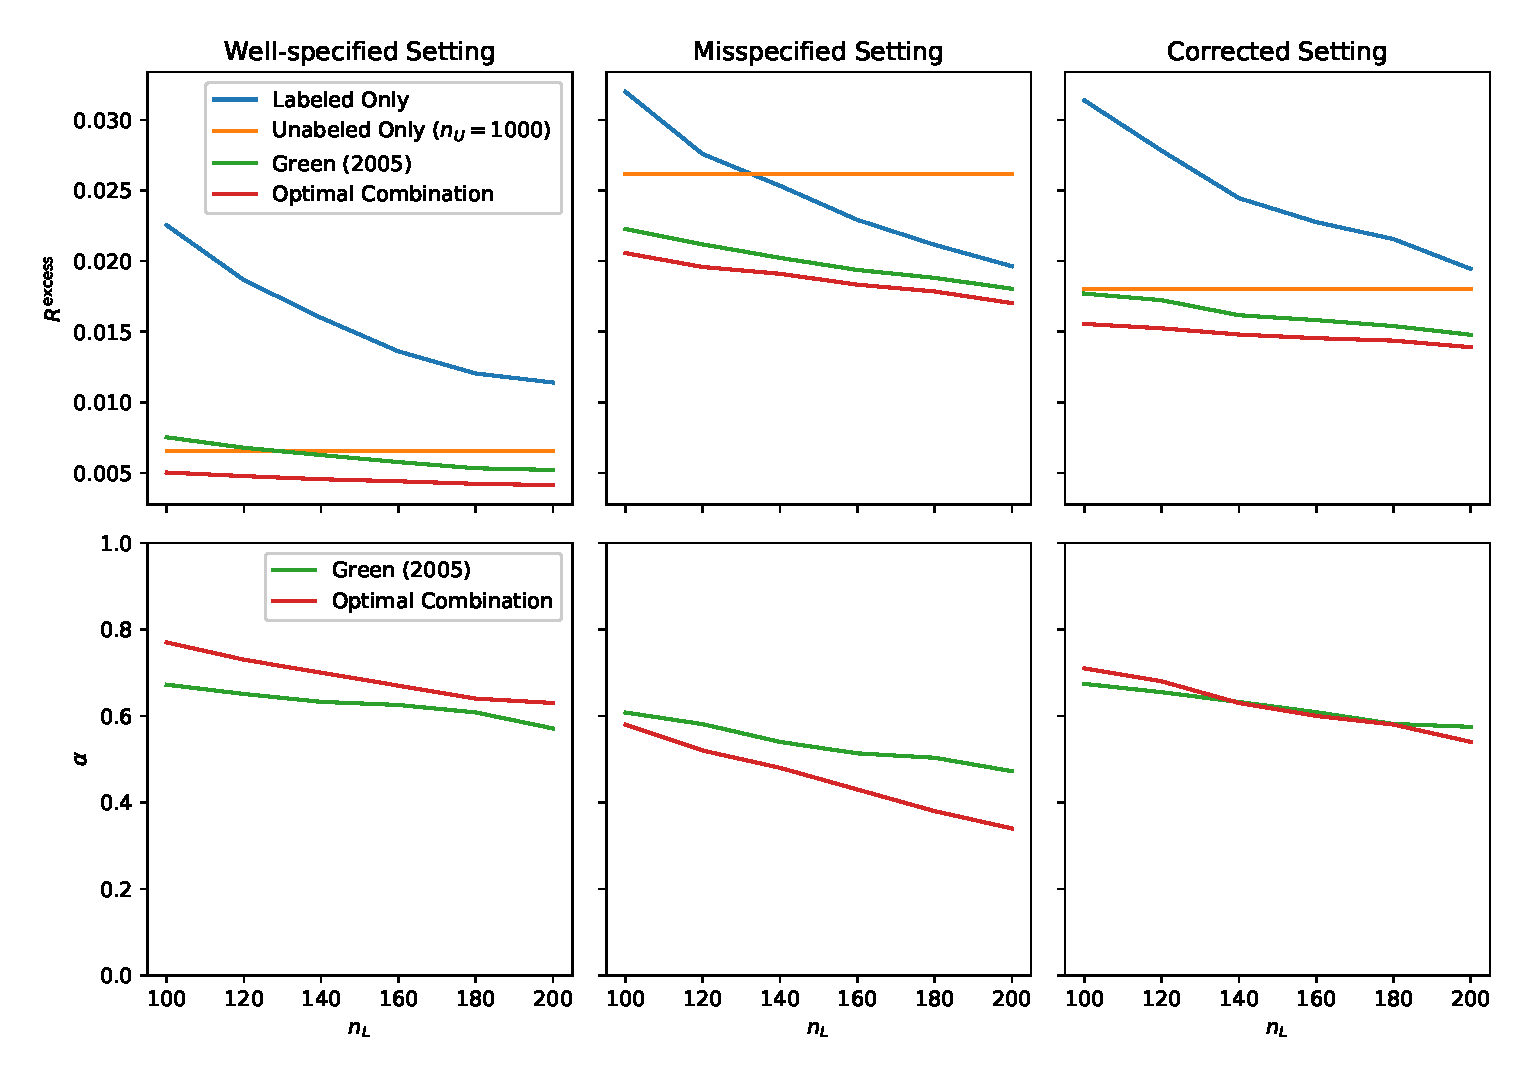
\includegraphics[width=.6\textwidth]{eps_figures/combined_with_alphas.eps}
    %
    \caption{Excess generalization error and associated combination weight $\alpha$ for an optimally weighted combination of labeled and unlabeled estimators, and a combination weighted according to \cite{GreenStrawderman2001} across the well-specified (left), misspecified (center), and corrected (right) settings. The number of unlabeled points is fixed at $n_U=1000$.}
    \label{fig:combined_with_alphas}
\end{figure}

\subsection{Real-World Case Study: Weak Supervision}

We discuss the weak supervision dataset we create and clarify the details of our experimental protocol for the real-world case study.

\paragraph{Creating a weak supervision dataset}

In weak supervision, soft labels from latent variable estimation are used as an alternative to a hand-labeled dataset. The sources used are usually heuristics which incorporate domain-specific knowledge about a particular task and can be acquired relatively cheaply. For our real-world case study, we choose the simple sentiment analysis task of classifying IMDB reviews as positive or negative. Our sources are defined simply: for a collection of positive sentiment words, output ``yes'' if the word appears in the review and ``no'' otherwise; for a collection of negative sentiment words, similarly output ``no'' if the word appears and ``yes'' otherwise. The specific words used and their sentiments are reported in \autoref{tab:imdb_words}. We select these words because they are empirically predictive, appear relatively frequently in reviews and are intuitively associated with positive/negative reviews.

\begin{table}[t]
\vskip 0.15in
\renewcommand{\arraystretch}{1.25} % Default value: 1
\begin{center}
\begin{small}
\begin{tabular}{l|cccccccccccccr}
\hline
Word & love & like & good & great & best & excellent & terrible & worst & bad & better & could & would \\
\hline
Sentiment & + & + & + & + & + & + & - & - & - & - & - & - \\
\hline
\end{tabular}
\end{small}
\end{center}
\vskip -0.1in
\caption{The words used as sources for the real-world weak supervision task of classifying IMDB reviews as positive or negative.}
\label{tab:imdb_words}
\end{table}

\paragraph{\autoref{fig:real_biases_data_value_ratio} and \autoref{tab:real_combo}: Experiments with real data} We measure excess generalization error, the data value ratio and the performances of combined estimators for the real-world dataset. Our protocols for these experiments mirror those we used for synthetic datasets, with two key differences: (1) for each trial, we sample points uniformly from the training set of 40,000 points, since we cannot sample directly from the distribution and (2) we measure generalization error on the test set, since we cannot compute the expected generalization error directly.



%\subsubsection*{Author Contributions}
%If you'd like to, you may include  a section for author contributions as is done
%in many journals. This is optional and at the discretion of the authors.

%\subsubsection*{Acknowledgments}
%Use unnumbered third level headings for the acknowledgments. All
%acknowledgments, including those to funding agencies, go at the end of the paper.

\end{document}



% If your paper is accepted, change the options for the package
% aistats2021 as follows:
%
%\usepackage[accepted]{aistats2021}
%
% This option will print headings for the title of your paper and
% headings for the authors names, plus a copyright note at the end of
% the first column of the first page.

% If you set papersize explicitly, activate the following three lines:
%\special{papersize = 8.5in, 11in}
%\setlength{\pdfpageheight}{11in}
%\setlength{\pdfpagewidth}{8.5in}

% If you use natbib package, activate the following three lines:
%\usepackage[round]{natbib}
%\renewcommand{\bibname}{References}
%\renewcommand{\bibsection}{\subsubsection*{\bibname}}

% If you use BibTeX in apalike style, activate the following line:
%\bibliographystyle{apalike}


% If your paper is accepted and the title of your paper is very long,
% the style will print as headings an error message. Use the following
% command to supply a shorter title of your paper so that it can be
% used as headings.
%
%\runningtitle{I use this title instead because the last one was very long}

% If your paper is accepted and the number of authors is large, the
% style will print as headings an error message. Use the following
% command to supply a shorter version of the authors names so that
% they can be used as headings (for example, use only the surnames)
%
%\runningauthor{Surname 1, Surname 2, Surname 3, ...., Surname n}

% Supplementary material: To improve readability, you must use a single-column format for the supplementary material.




